% Created 2024-06-19 Wed 14:54
% Intended LaTeX compiler: pdflatex
\documentclass[10pt,a4paper,onecolumn,notitlepage,oneside,dvipdfmx]{article}
\usepackage{graphicx}
\usepackage{longtable}
\usepackage{wrapfig}
\usepackage{rotating}
\usepackage[normalem]{ulem}
\usepackage{amsmath}
\usepackage{amssymb}
\usepackage{capt-of}
\usepackage{hyperref}
\usepackage[newfloat]{minted}
\usepackage{fancyhdr}
\usepackage{amsmath}
\usepackage{amssymb}
\usepackage{bm}
\usepackage{color}
\usepackage{graphicx}
\usepackage{tikz}
\usepackage{wrapfig}
\setlength{\oddsidemargin}{-10mm}
\setlength{\topmargin}{-10mm}
\setlength{\textheight}{245mm}
\setlength{\textwidth}{180mm}
\renewcommand{\figurename}{Fig.}
\renewcommand{\tablename}{Tab.}
\newcommand{\Figure}[1]{\figurename{\ref{#1}}}
\newcommand{\Table} [1]{\tablename {\ref{#1}}}
\makeatletter
\newcommand{\figcaption}[1]{\def\@captype{figure}\caption{#1}}
\newcommand{\tblcaption}[1]{\def\@captype{table}\caption{#1}}
\pagestyle{fancy}
\lhead{\@leftheader}
\rhead{\@rightheader}
\newcommand{\leftheader} [1]{\def\@leftheader{#1}}
\newcommand{\rightheader}[1]{\def\@rightheader{#1}}
\leftheader{グループゼミ資料}
\rightheader{Ver.Ka}
\renewcommand{\maketitle}{%
\begin{center}{\Large \@title}\end{center}%
\begin{flushright}\@author\\ \@date\end{flushright}%
\hrulefill\\}
\usepackage{multirow}
\usepackage{subcaption}
\usepackage{lscape}
\usepackage{ascmac}
\usepackage{bm}
\usepackage{here}
\usepackage{latexsym}
\usepackage{algorithm}
\usepackage{algpseudocode}
\usepackage{url}
\usetikzlibrary{arrows,automata}
\algnewcommand\algorithmicforeach{\textbf{for each}}
\algdef{S}[FOR]{ForEach}[1]{\algorithmicforeach\ #1\ \algorithmicdo}
\DeclareMathOperator*{\argmax}{arg\,max}
\DeclareMathOperator*{\argmin}{arg\,min}
\author{Vincent Conus}
\date{2024/06/19}
\title{Ender-3 S1 Pro: 使う方法ガイド\\\medskip
\large 稲垣研究室、南山大学}
\hypersetup{
 pdfauthor={Vincent Conus},
 pdftitle={Ender-3 S1 Pro: 使う方法ガイド},
 pdfkeywords={},
 pdfsubject={},
 pdfcreator={Emacs 30.0.50 (Org mode 9.6.15)}, 
 pdflang={English}}
\begin{document}

\maketitle
\tableofcontents

\section{初めに}
\label{sec:orga813bd2}
「Ender-3 S1 Pro」と言うの機会は様々な種類のポリマー材料を用いて印刷できる積層造形装置です。

\begin{figure}[htbp]
\centering
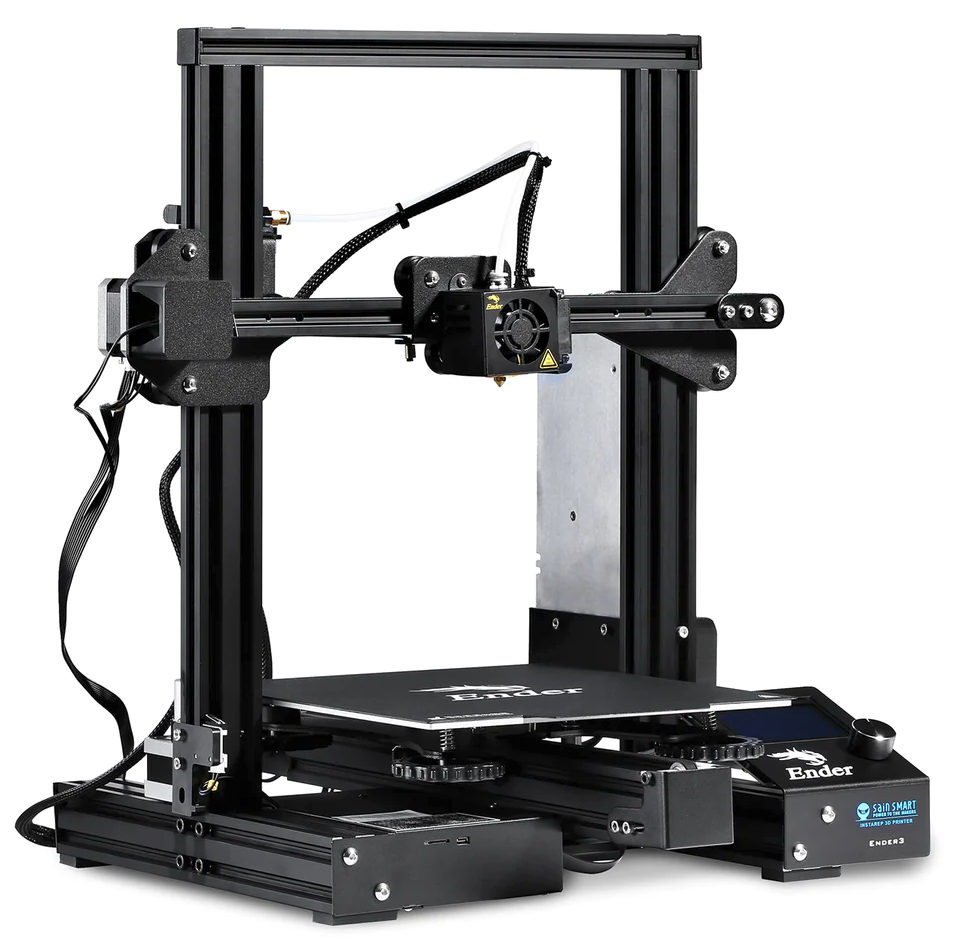
\includegraphics[width=0.7\textwidth]{img/ender3.png}
\end{figure}

\subsection{練習:Benchy}
\label{sec:orgf429a9d}
\begin{figure}[htbp]
\centering
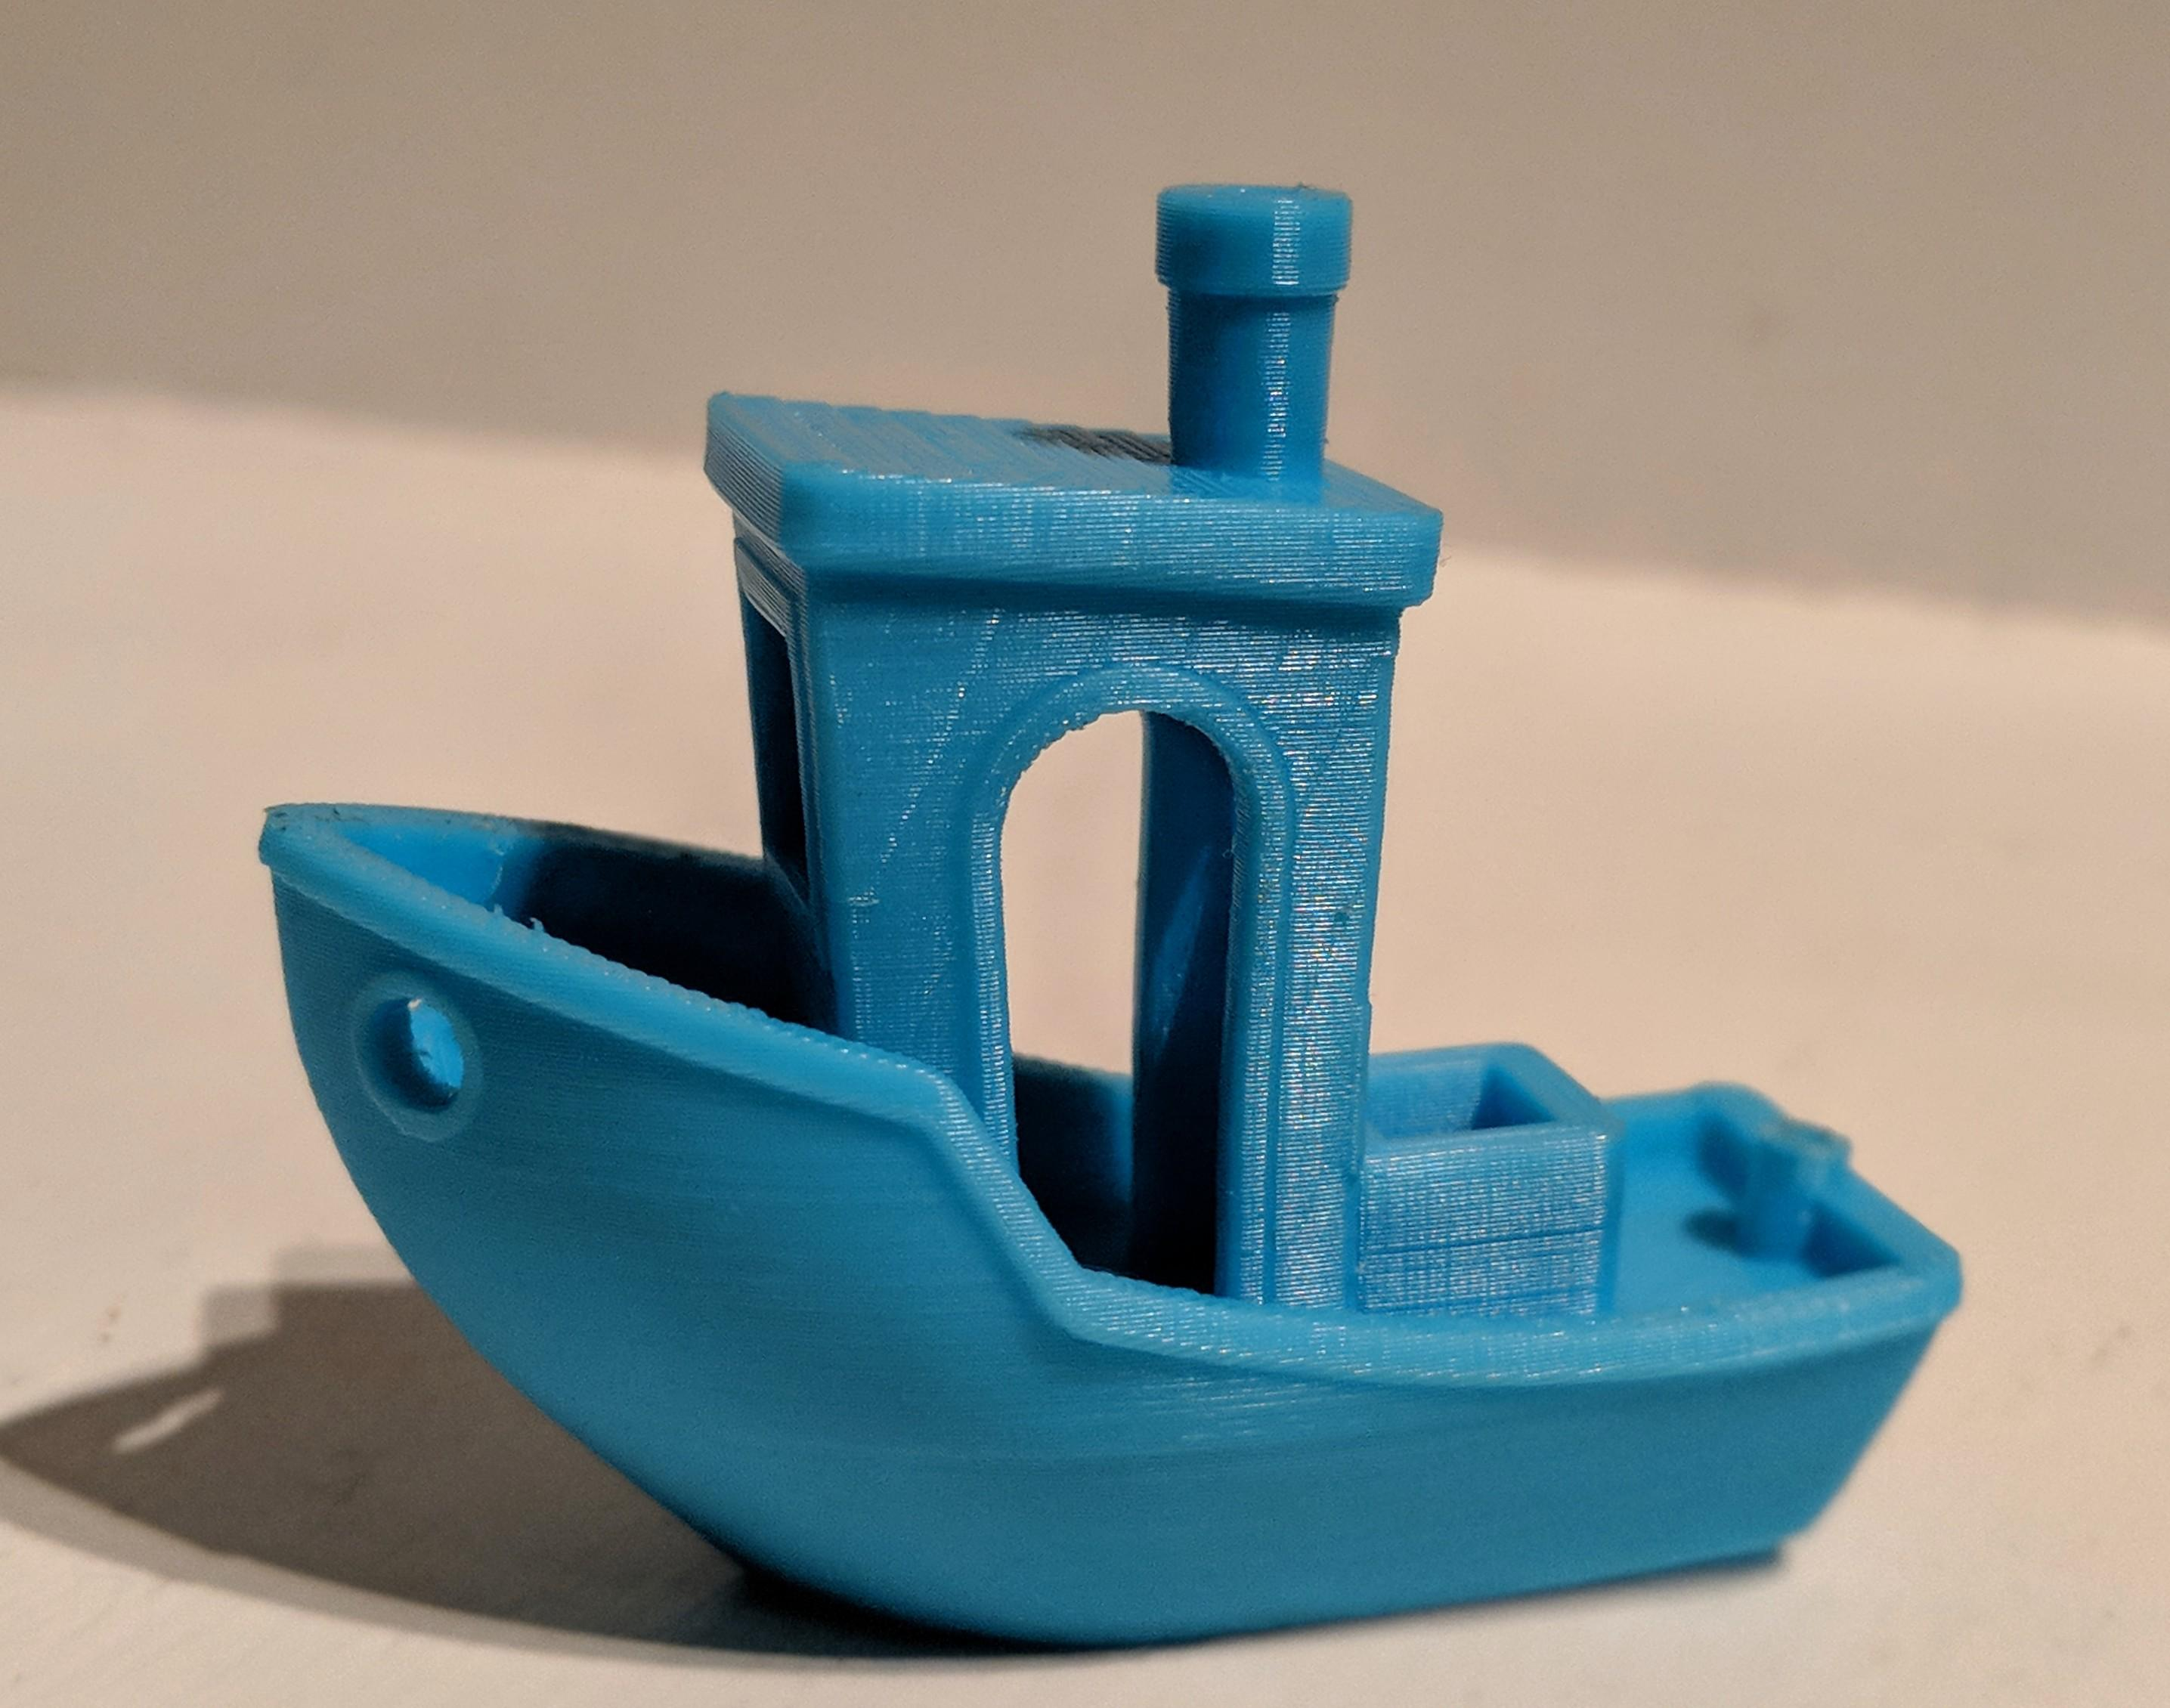
\includegraphics[width=0.7\textwidth]{img/benchy.jpg}
\caption{かわいい船}
\end{figure}


\section{スライシング}
\label{sec:org2db262d}

\section{プリンチング}
\label{sec:orgacab8a9}

\section{整備助言}
\label{sec:orgd940f5d}

\subsection{湿気}
\label{sec:org86f712d}
3Dプリンター用ラメントスプールは、一般的に湿気に弱い。
もし長期間使用しない場合は、プリンターから取り出して箱に戻し、理想的にはケイ酸塩を入れた袋を中に入れて保管してください。
\end{document}
